\usepackage[utf8]{inputenc}
\usepackage[T1]{fontenc}
\usepackage[hidelinks]{hyperref}
\usepackage{graphicx}
\graphicspath{ {figures/}
} 

\chapter{Recursive Make Considered Harmful}

\section{Introduction}

\hyperref[This]{''http://aegis.sourceforge.net/auug97.pdf''} paper was written by Peter Miller of the Australian Organisation for Unix,
Linux, and Open Source Professionals in 1997. It discusses the problem of 
"unacceptable large" build times on large UNIX projects, even when make small 
changes. The author attributes the problem to the use of recursive makes. Specifically,
the artificial partitioning of the build into separate subsets which leads to incomplete
make files.

According to the author, the problem is not with Make itself, rather the input going into
make - \textit{Garbage In Garbage Out}. 


\section{What is a Recursive Make?}

Projects that make use of recursive makes use a hierarchy of direcetories containing 
source files for the module which make up the project, where each sub-directory
contains a Makefile describing the rules and instructions for the make program.

The complete build is done by setting the top-level Makefile to change directory into
each of the sub-directories and recursively invoke the \textit{make} program.

This hierarchy can be nested arbitrarily deep, typically two- and three-level structures.

%Include image of recursive makefile structure
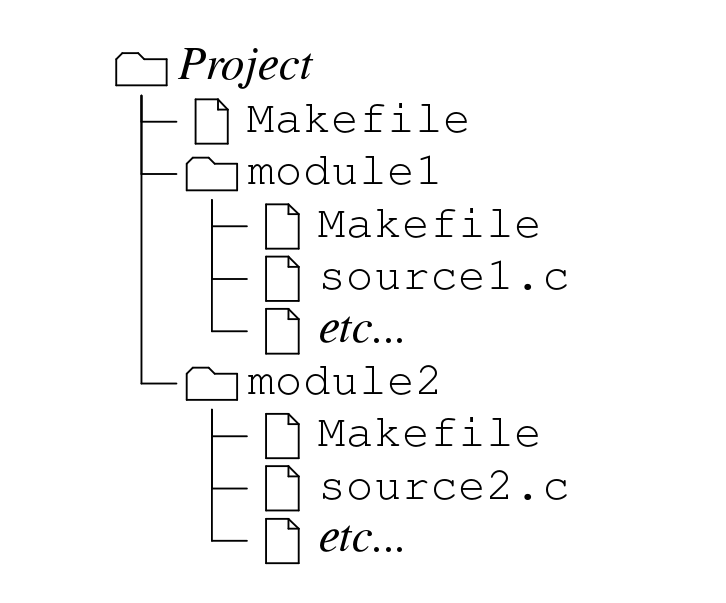
\includegraphics[width=3cm]{structure}
\subsection{Problems}
\begin{enumerate}
\item Difficult to get order of recursion into sub-directories correct - unstable and 
often needs tweaking.
\item Often necessary to do more than one pass over sub-directories - increases build times.
\item Some dependency information is omitted to avoid unreasonable build times.
\item Inter-directory dependencies often omitted or too hard to express, so Makefiles written to 
\textit{over} build to ensure nothing is left out.
\item Inaccurate dependencies lead to the product unable to build cleanly.
\end{enumerate}

\section{What "Make" Does and How It Works}

Give it a set of rules for how to construct things, and a target to be constructed. Rules 
are decomposed into pair-wise ordered dependencies between files. Make takes these files 
and determines how to build the given target. It does this by constructing a
\textit{Directed Acyclic Graph} (DAG).

An example project structure:
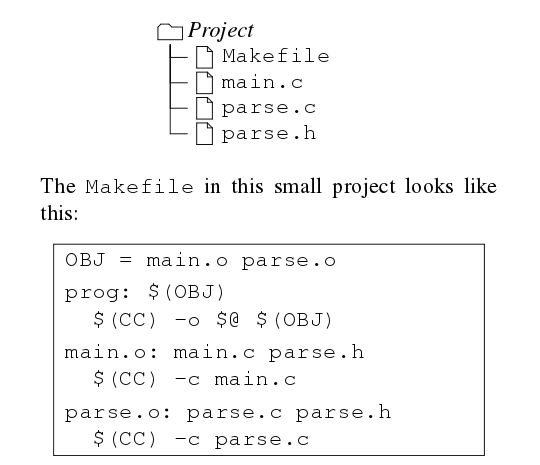
\includegraphics[width=3cm]{simpleproject}

Corresponding Directed Acyclic Graph:
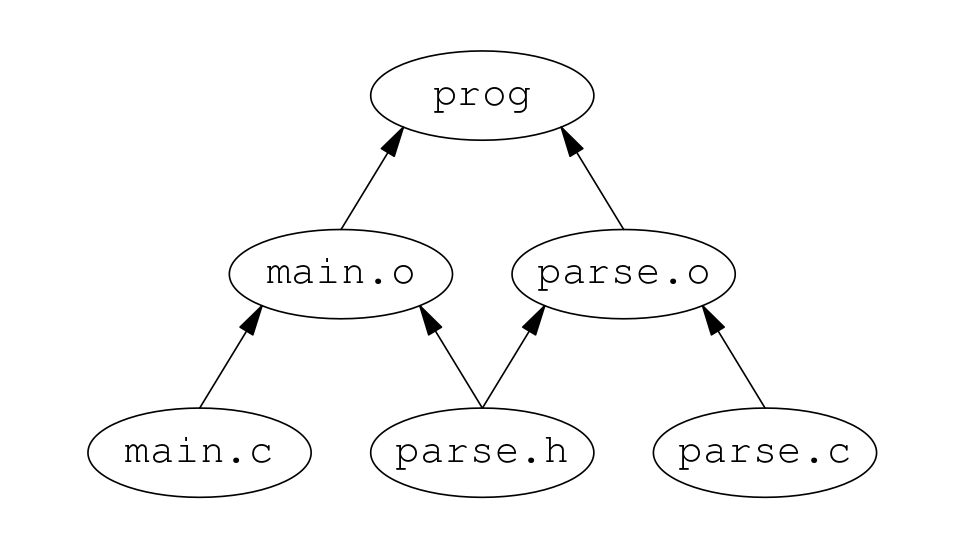
\includegraphics[width=3cm]{dag}

Object files are dependent on the include files \textit{(.h)} even though source files \textit{(.c)} do the including.
This is because if an include file changes, it is the object files that are out-of-date, not the 
source files.

After make has created the DAG, it performs a \textit{postorder} traversal of the DAG. Dependencies are 
visited first. It looks at the last modified of each file, higher files are considered out-of-date if
any of the lower files they depend upon are younger.

Using recursive makes is problematic because it affects both phases: it causes make to construct an
inaccurate DAG, and it forces make to traverse the DAG in an inappropriate order.

Incomplete DAG from recursive make:
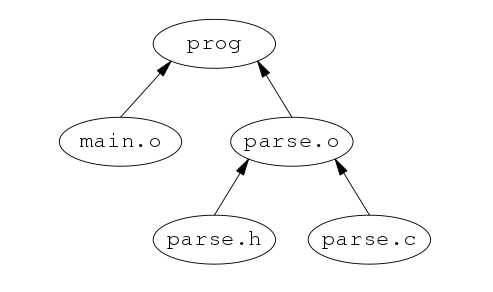
\includegraphics[width=3cm]{incompletedag}

Files are interdependent. Using make recursively means that files created for the next process whilst
unaware of problems such as out-of-date. These out-of-date files are then used as input for later stages
(which \textit{are} aware of being out-of-date), leading to compatibility problems.

\section{Solution}

Use one Makefile for an entire project instead of breaking it up.

\begin{quote}
It is not the recursion itself which is harmful, it is the crippled Makefiles which are used
in the recursion which are wrong.
\end{quote}

It may sound counter-intuitive to have a single Makefile, however the author says that by using \textit{include}
statements, the Makefile is instructed to suspend reading the current one and go to another before continuing.

\section{Conclusion}

This paper is not a typical example of scientific paper, it reads more like a
technical paper. It addresses a real problem related to the misuse of Make to build large projects. The paper 
goes beyond the tutorial like presentations of Make which only state features of the tool and its syntax,
these details can be found in the manuals and
readme files.

Make was designed with the idea that DAG representing the dependency is known beforehand, in such a case 
Make will walk through the dependency graph, recompiling the source files that have been updated and the object 
files that depend on those sources. 

When Makefiles became long and complex the approach proposed to deal with this complexity was to have multiple
makefile distributed over project directory tree breaking the whole idea of Make having a global of view of the
overall dependency of the project. This is turn made the build of large project sometimes unpredictable and 
forces the Makefiles writer either to build too much (multiple traversal of the DAG, or clean the entire project tree)
which does not help to reduce build time of large projects. The rest of the details are only relevant to a person 
who will be facing the problem of creating Manually a makefile for a large software project.